

\begin{figure}

        \textbf{\rotatebox[origin=c]{90}{\hspace{-7.5em} MSE \hspace{2.5em} y(t) \hspace{1.5em} x(t)}}
        \begin{subfigure}{\textwidth}
            \centering
    
            \textbf{5 segments}\hspace{12em}\textbf{6 segments}
            
            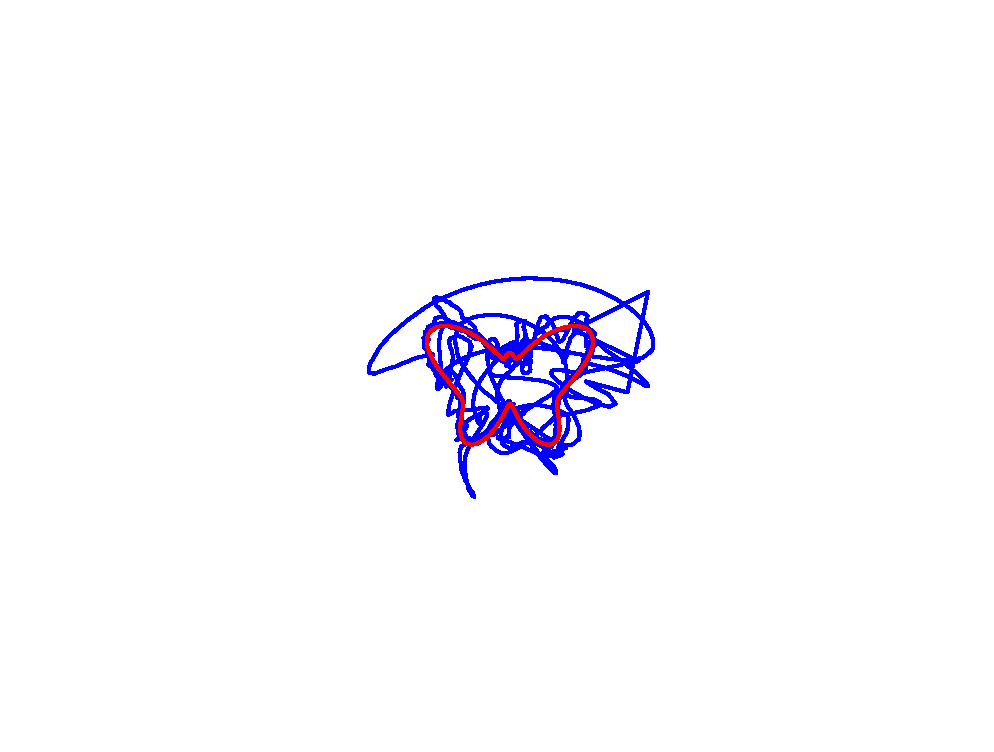
\includegraphics[trim=5cm 4cm 5cm 4cm, clip=true,height=0.15\linewidth]{Figures/Fig_T6/ImprovP/ST_T2_Seg5_Var_Trajectory.eps}
            \hspace{9em}
            \includegraphics[trim=5cm 4cm 5cm 4cm, clip=true,height=0.15\linewidth]{Figures/Fig_T6/ImprovP/ST_T2_Seg6_Var_Trajectory.eps}
            %trim=1cm 0cm 0cm 0cm, clip=true,
            
            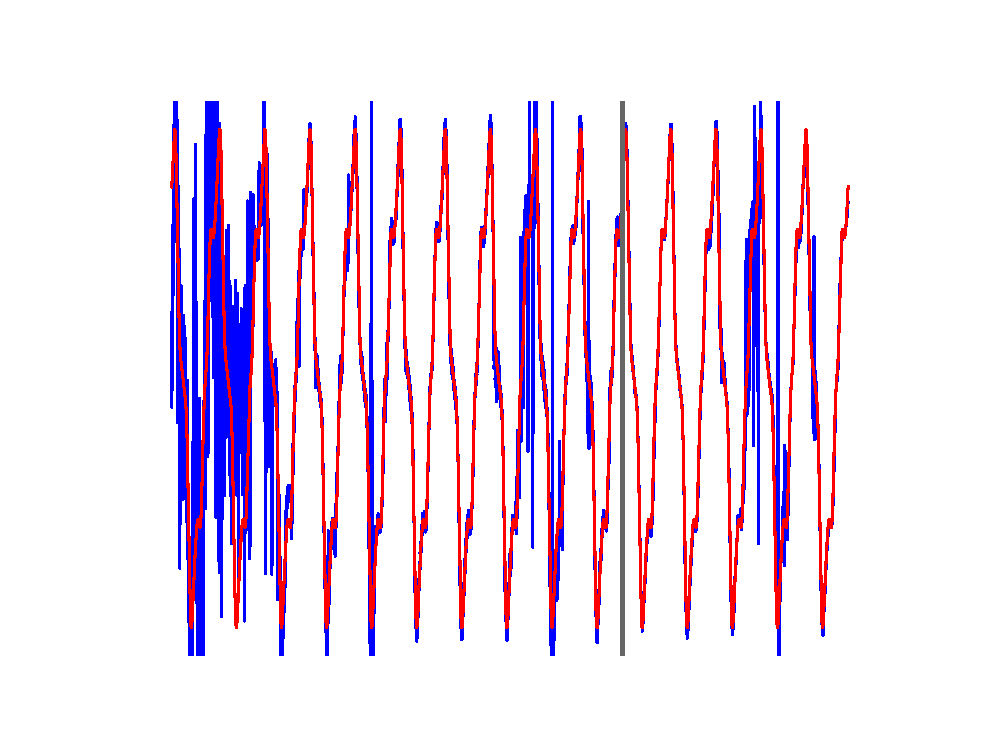
\includegraphics[trim=2cm 1cm 2cm 1cm, clip=true,height=0.1\linewidth,width=.45\linewidth]{Figures/Fig_T6/ImprovP/ST_T2_Seg5_Var_CoordinateX.eps} 
            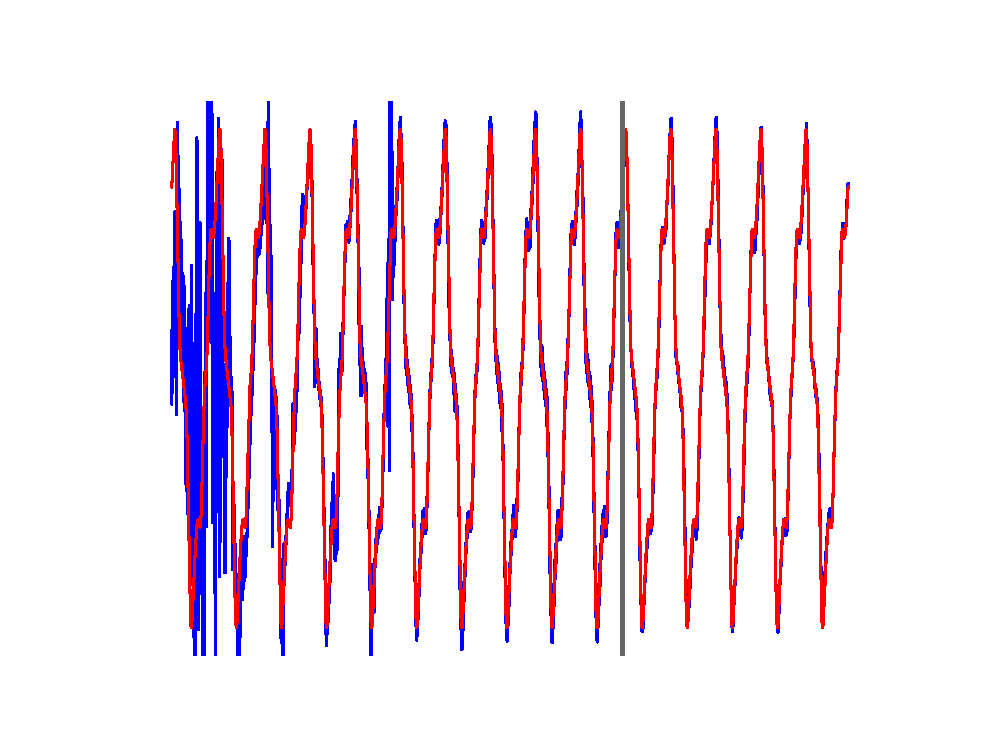
\includegraphics[trim=2cm 1cm 2cm 1cm, clip=true,height=0.1\linewidth,width=.45\linewidth]{Figures/Fig_T6/ImprovP/ST_T2_Seg6_Var_CoordinateX.eps}       

            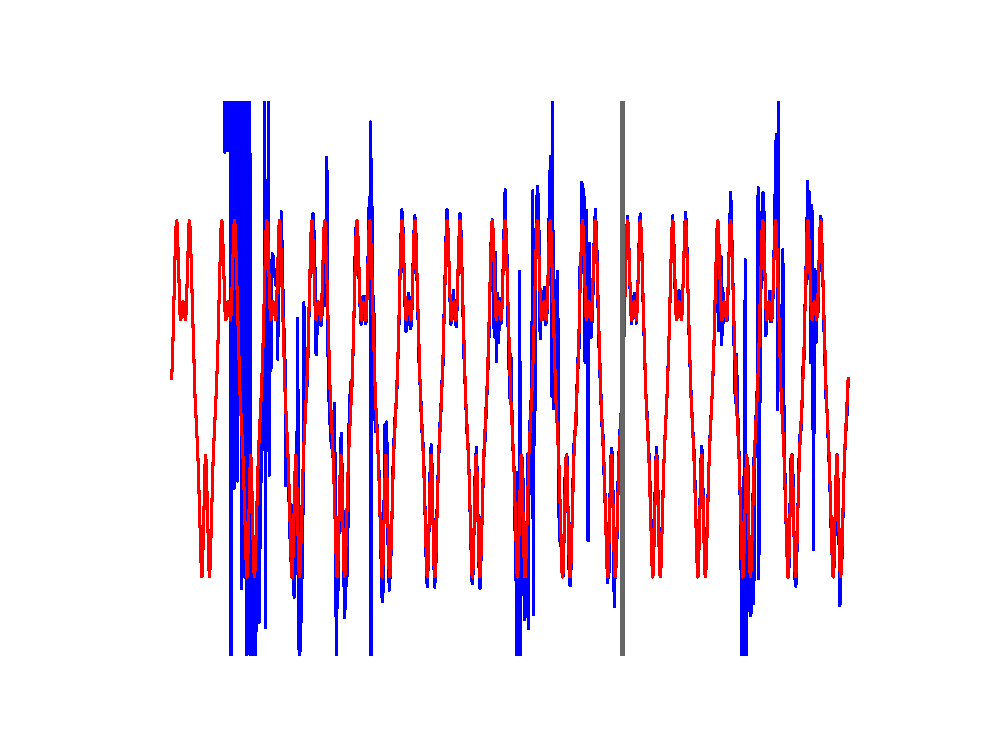
\includegraphics[trim=2cm 1cm 2cm 1cm, clip=true,height=0.1\linewidth,width=.45\linewidth]{Figures/Fig_T6/ImprovP/ST_T2_Seg5_Var_CoordinateY.eps}    
            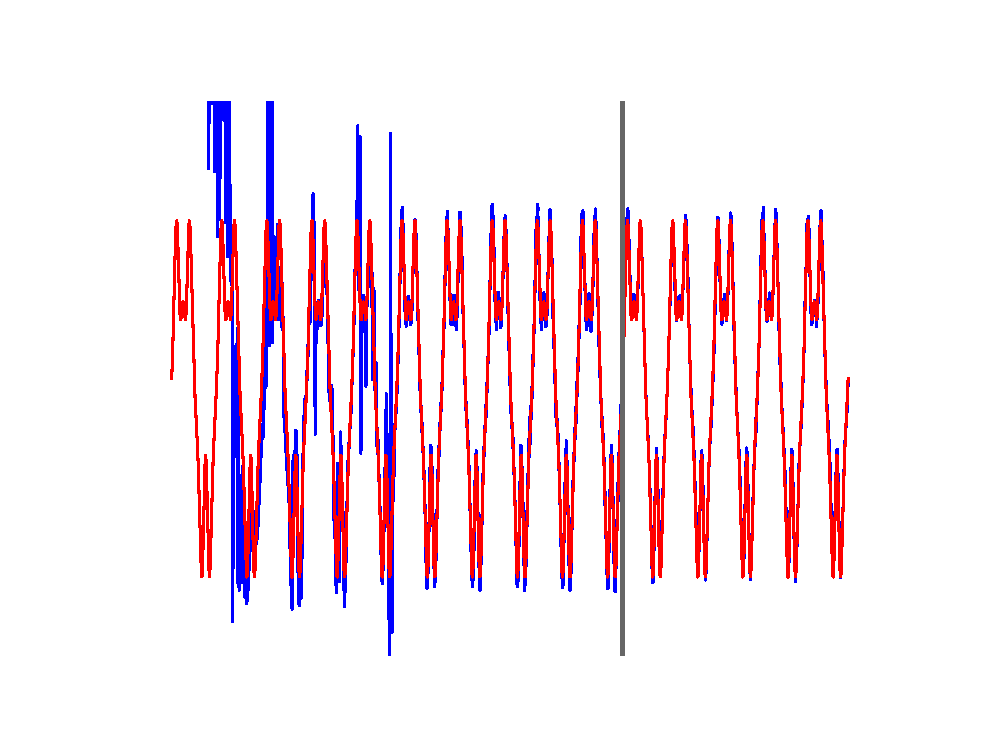
\includegraphics[trim=2cm 1cm 2cm 1cm, clip=true,height=0.1\linewidth,width=.45\linewidth]{Figures/Fig_T6/ImprovP/ST_T2_Seg6_Var_CoordinateY.eps} 

            \hspace{-1em}
            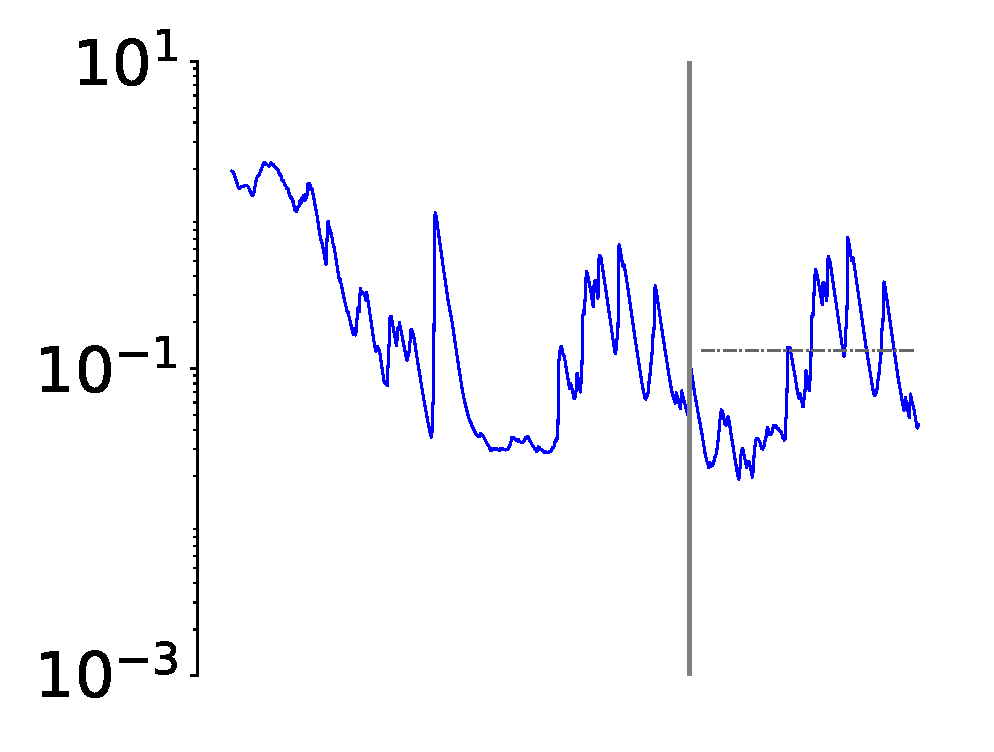
\includegraphics[height=0.15\linewidth,width=.45\linewidth]{Figures/Fig_T6/ImprovP/ST_T2_Seg5_Var_MSE.eps}
            \hspace{0em}
            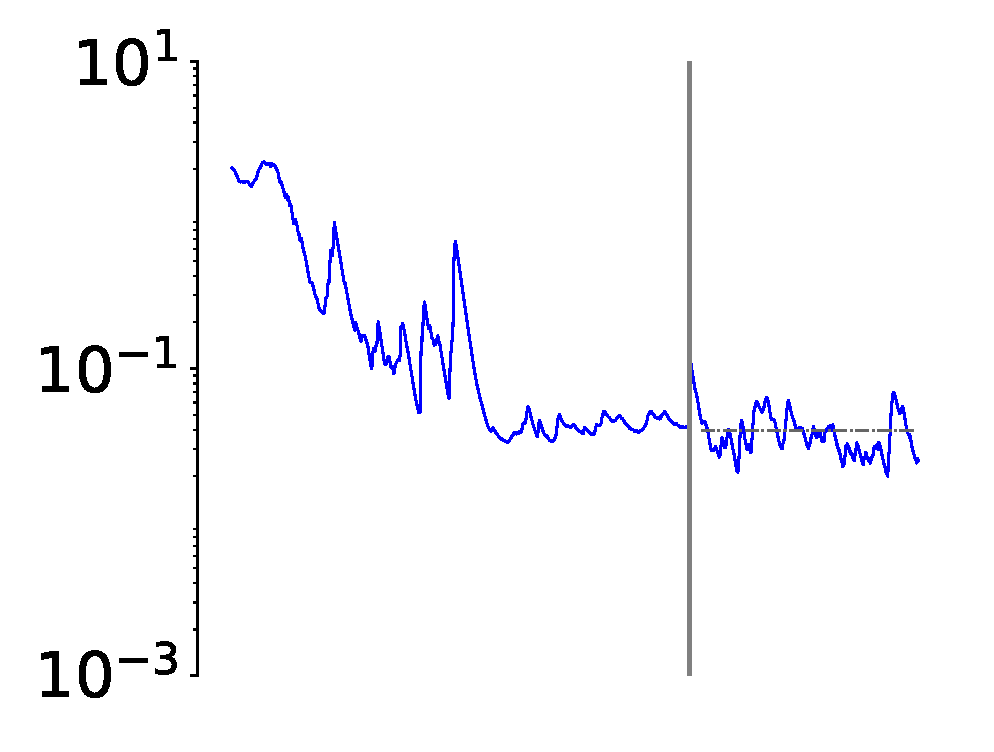
\includegraphics[height=0.15\linewidth,width=.45\linewidth]{Figures/Fig_T6/ImprovP/ST_T2_Seg6_Var_MSE.eps}

        \end{subfigure}
        
        \textbf{\rotatebox[origin=c]{90}{\hspace{-7.5em} MSE \hspace{2.5em} y(t) \hspace{1.5em} x(t)}}
        \begin{subfigure}{\textwidth}
            \centering
    
            \textbf{7 segments}\hspace{12em}\textbf{8 segments}
            
            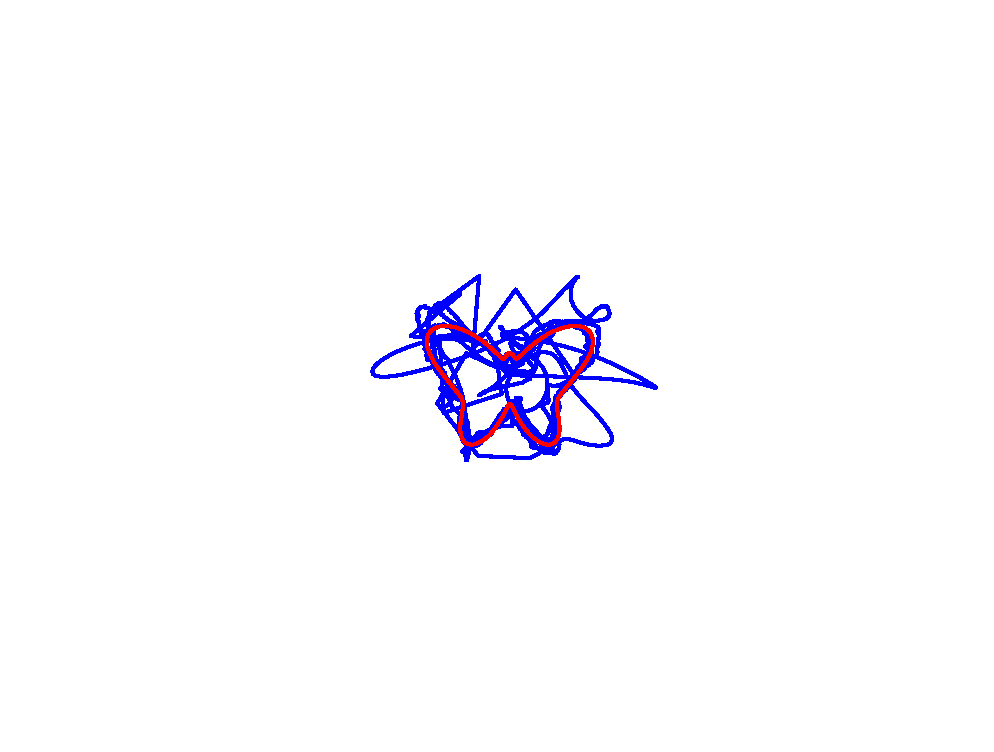
\includegraphics[trim=5cm 4cm 5cm 4cm, clip=true,height=0.15\linewidth]{Figures/Fig_T6/ImprovP/ST_T2_Seg7_Var_Trajectory.eps}
            \hspace{9em}
            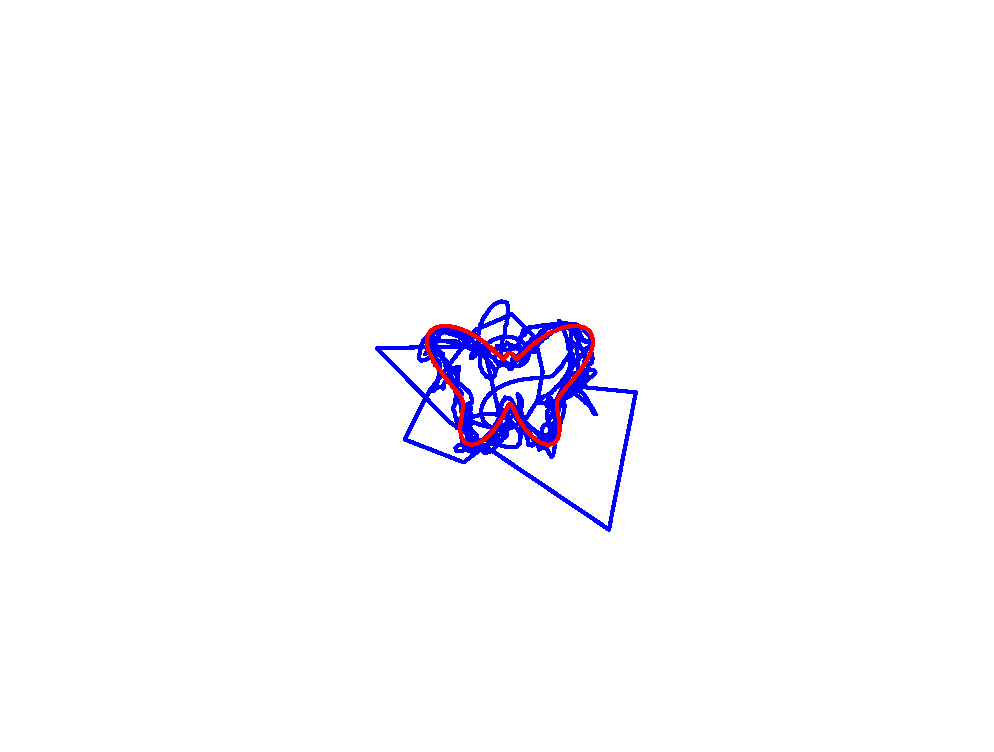
\includegraphics[trim=5cm 4cm 5cm 4cm, clip=true,height=0.15\linewidth]{Figures/Fig_T6/ImprovP/ST_T2_Seg8_Var_Trajectory.eps}
            %trim=1cm 0cm 0cm 0cm, clip=true,
            
            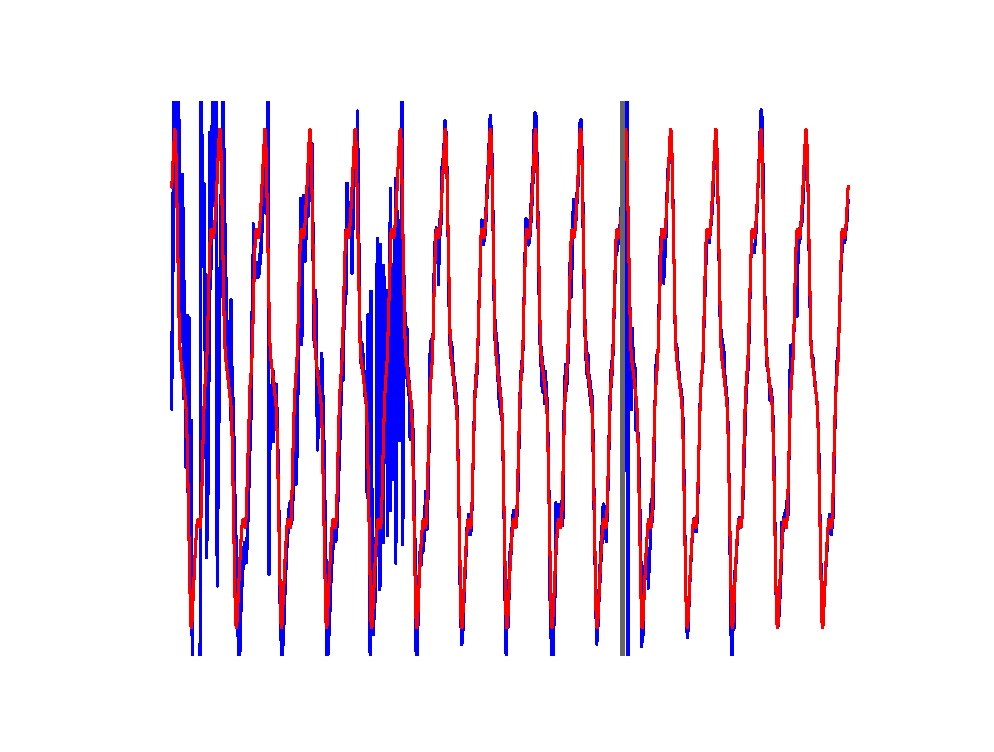
\includegraphics[trim=2cm 1cm 2cm 1cm, clip=true,height=0.1\linewidth,width=.45\linewidth]{Figures/Fig_T6/ImprovP/ST_T2_Seg7_Var_CoordinateX.eps} 
            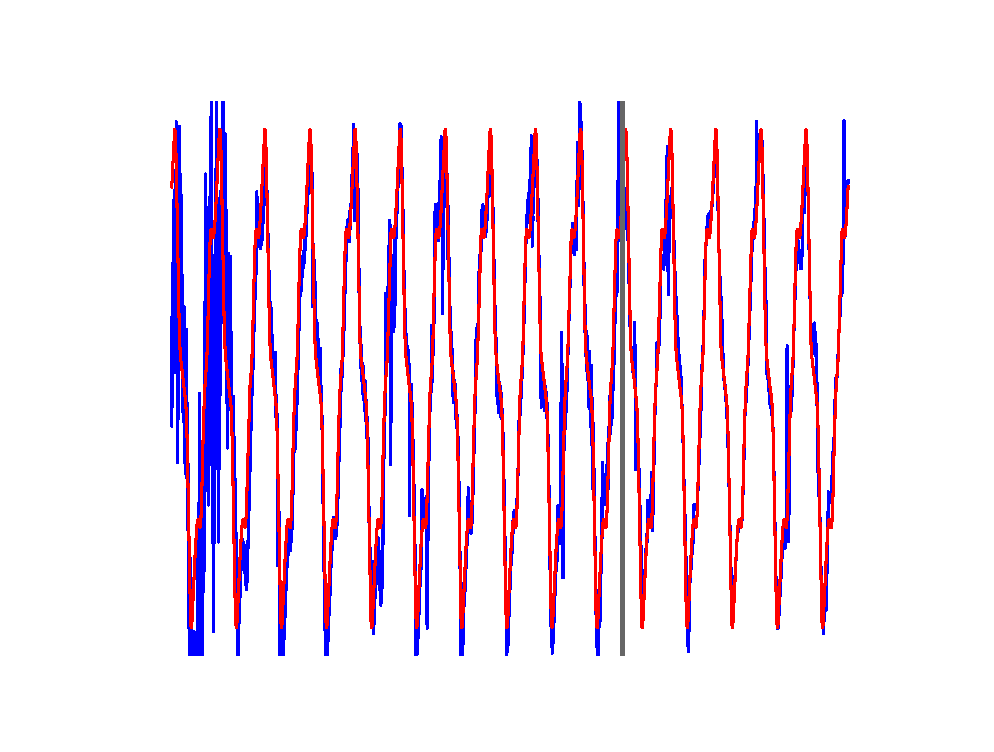
\includegraphics[trim=2cm 1cm 2cm 1cm, clip=true,height=0.1\linewidth,width=.45\linewidth]{Figures/Fig_T6/ImprovP/ST_T2_Seg8_Var_CoordinateX.eps}       

            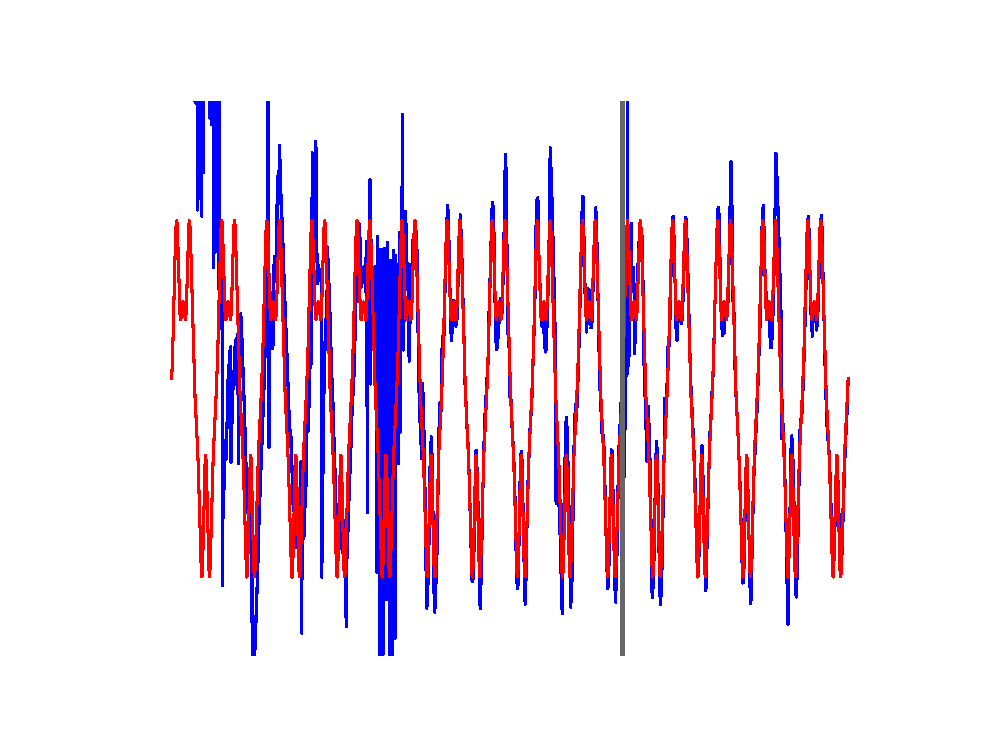
\includegraphics[trim=2cm 1cm 2cm 1cm, clip=true,height=0.1\linewidth,width=.45\linewidth]{Figures/Fig_T6/ImprovP/ST_T2_Seg7_Var_CoordinateY.eps}    
            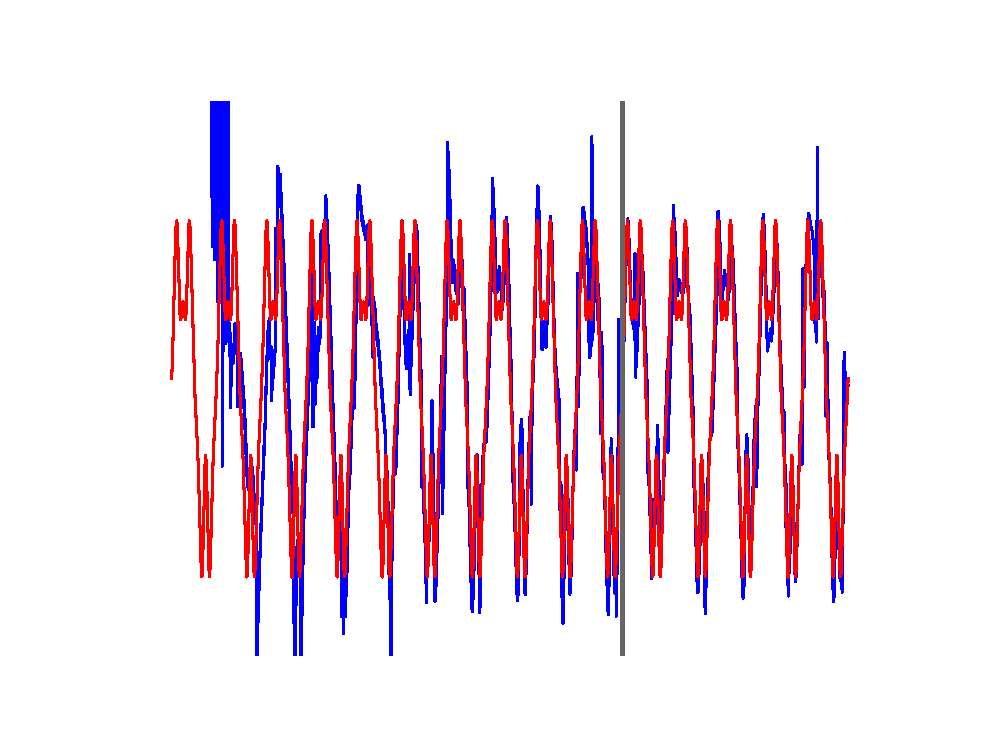
\includegraphics[trim=2cm 1cm 2cm 1cm, clip=true,height=0.1\linewidth,width=.45\linewidth]{Figures/Fig_T6/ImprovP/ST_T2_Seg8_Var_CoordinateY.eps} 

            \hspace{-1em}
            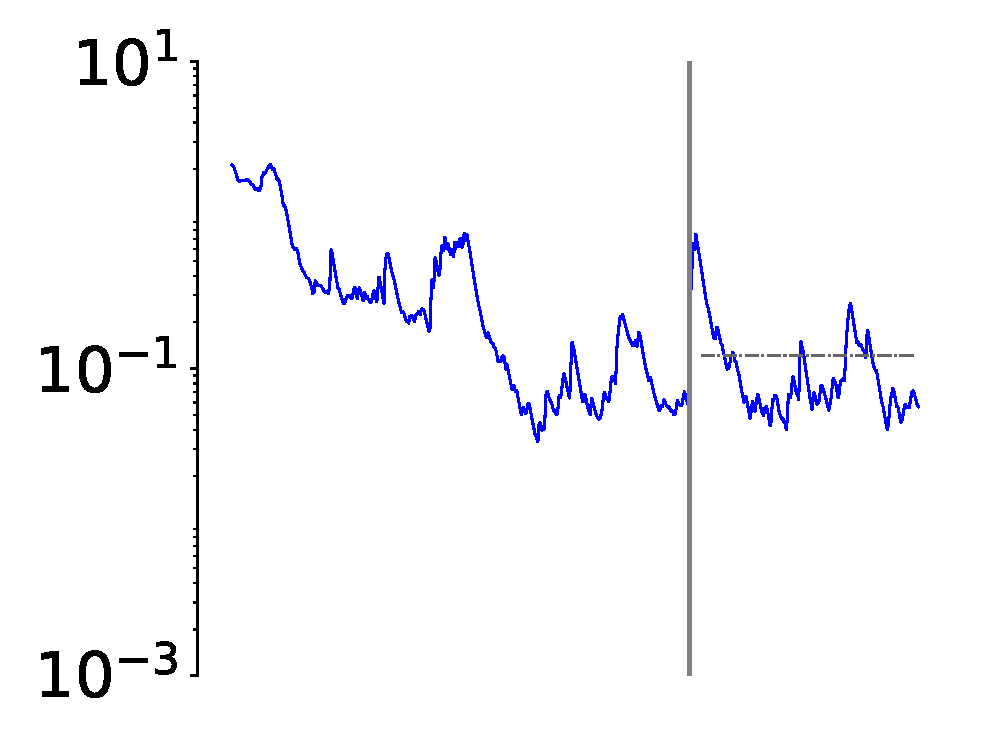
\includegraphics[height=0.15\linewidth,width=.45\linewidth]{Figures/Fig_T6/ImprovP/ST_T2_Seg7_Var_MSE.eps}
            \hspace{0em}
            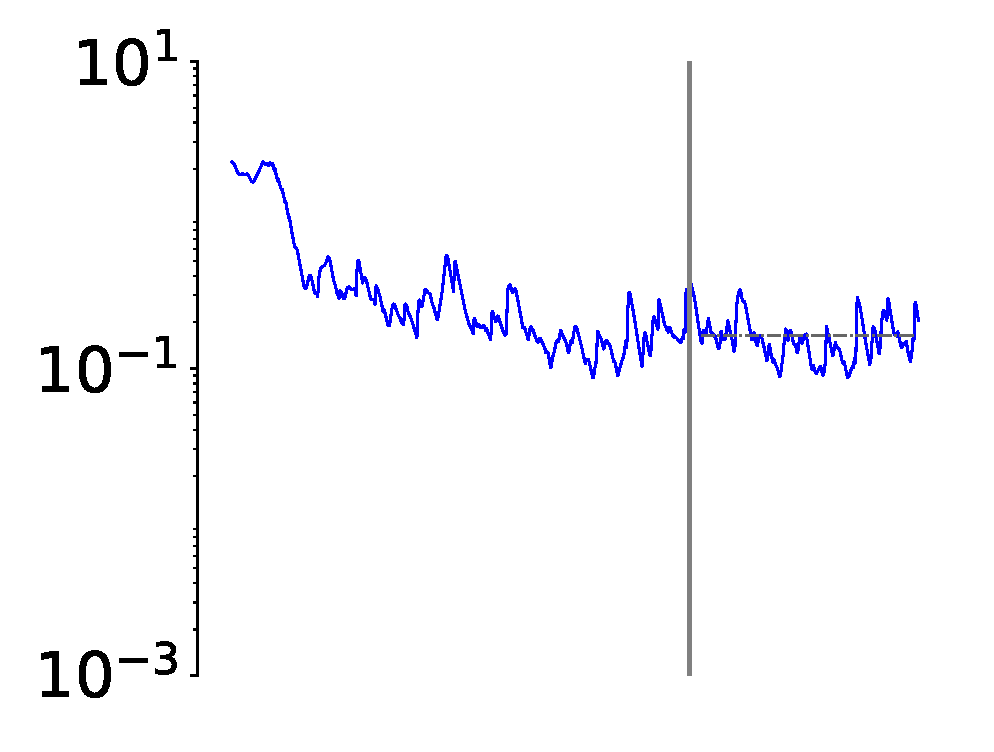
\includegraphics[height=0.15\linewidth,width=.45\linewidth]{Figures/Fig_T6/ImprovP/ST_T2_Seg8_Var_MSE.eps}
            
            
        \end{subfigure}
        
        \textbf{\rotatebox[origin=c]{90}{\hspace{-7.5em} MSE \hspace{2.5em} y(t) \hspace{1.5em} x(t)}}
        \begin{subfigure}{\textwidth}
            \centering
    
            \textbf{9 segments}\hspace{12em}\textbf{10 segments}
            
            
            
            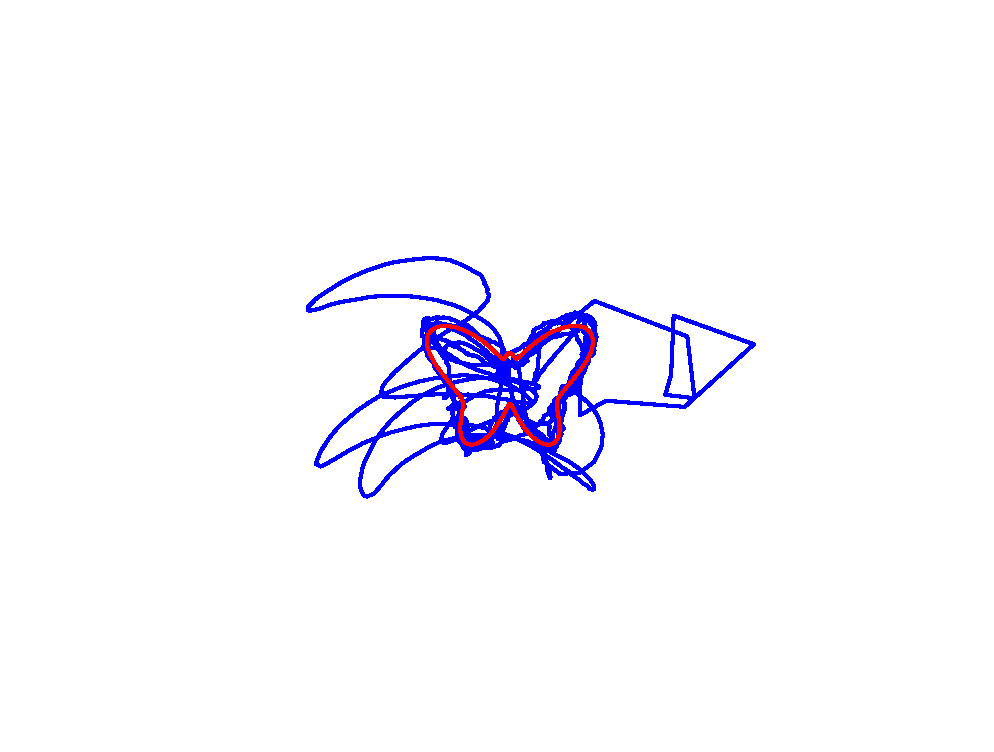
\includegraphics[trim=5cm 4cm 5cm 4cm, clip=true,height=0.15\linewidth]{Figures/Fig_T6/ImprovP/ST_T2_Seg9_Var_Trajectory.eps}
            \hspace{9em}
            \includegraphics[trim=5cm 4cm 5cm 4cm, clip=true,height=0.15\linewidth]{Figures/Fig_T6/ImprovP/ST_T2_Seg10_Var_Trajectory.eps}
            %trim=1cm 0cm 0cm 0cm, clip=true,
            
            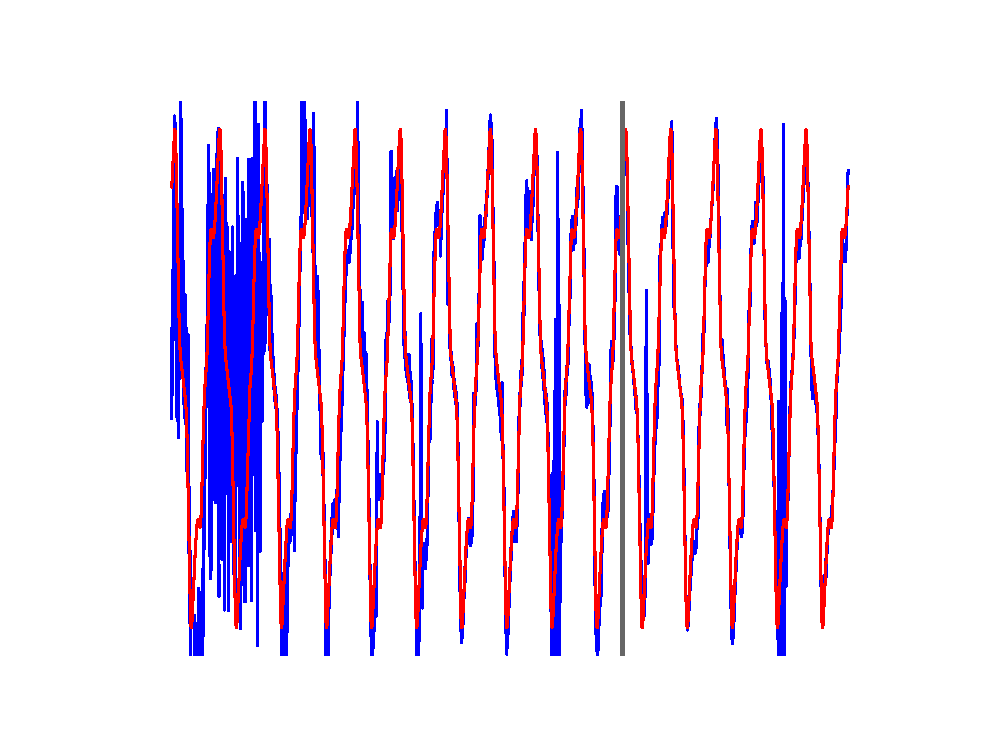
\includegraphics[trim=2cm 1cm 2cm 1cm, clip=true,height=0.1\linewidth,width=.45\linewidth]{Figures/Fig_T6/ImprovP/ST_T2_Seg9_Var_CoordinateX.eps} 
            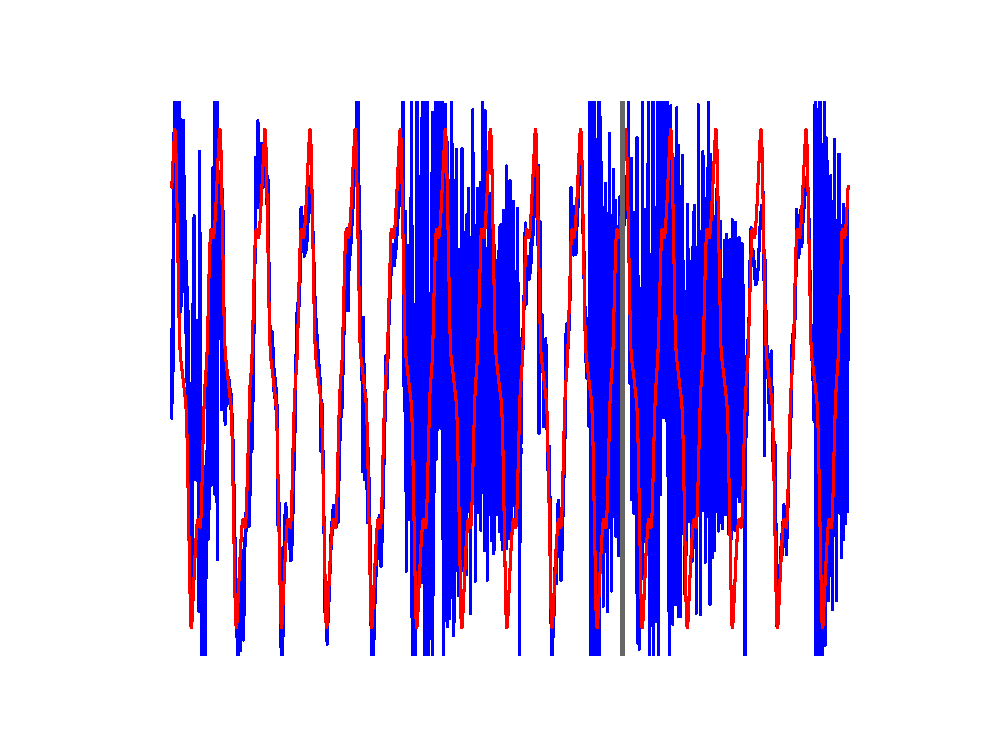
\includegraphics[trim=2cm 1cm 2cm 1cm, clip=true,height=0.1\linewidth,width=.45\linewidth]{Figures/Fig_T6/ImprovP/ST_T2_Seg10_Var_CoordinateX.eps}       

            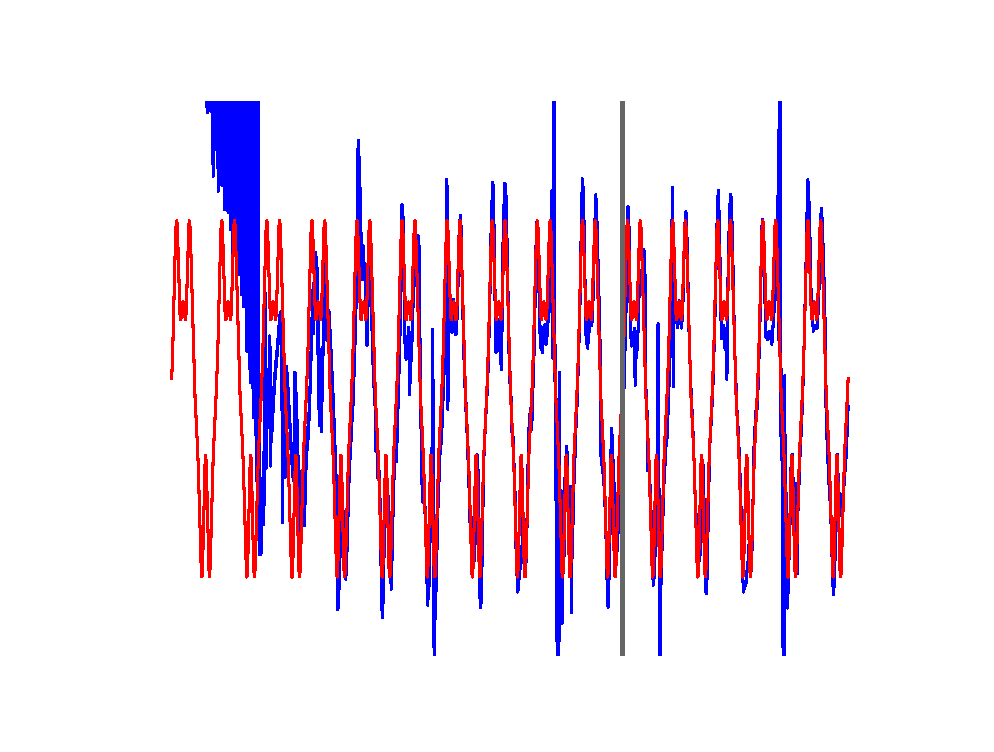
\includegraphics[trim=2cm 1cm 2cm 1cm, clip=true,height=0.1\linewidth,width=.45\linewidth]{Figures/Fig_T6/ImprovP/ST_T2_Seg9_Var_CoordinateY.eps}    
            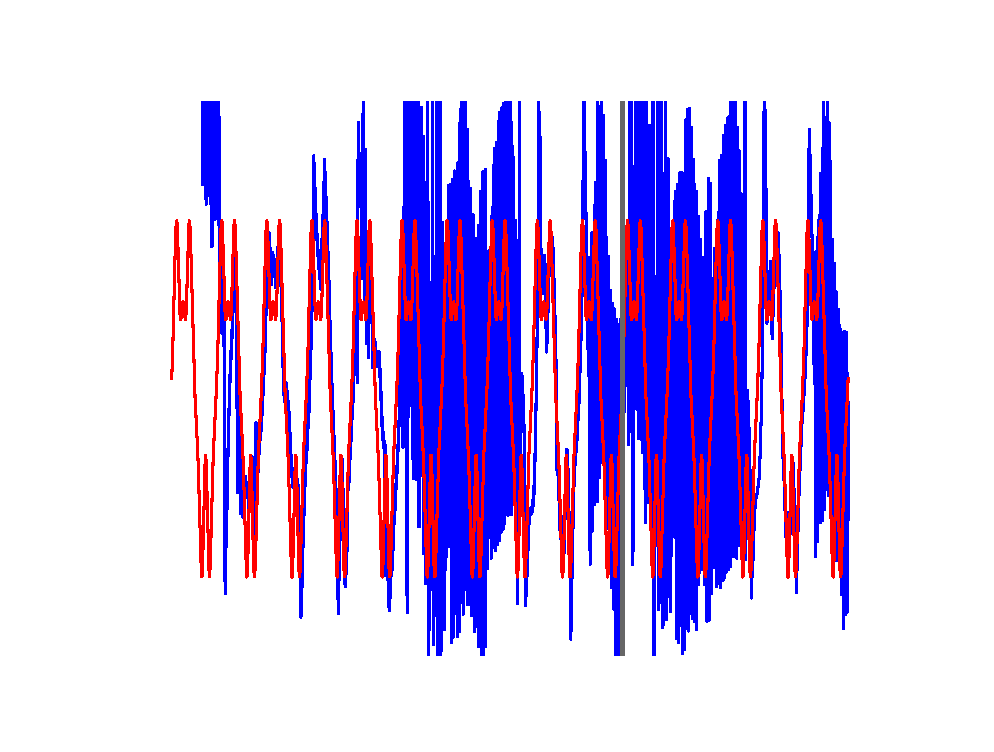
\includegraphics[trim=2cm 1cm 2cm 1cm, clip=true,height=0.1\linewidth,width=.45\linewidth]{Figures/Fig_T6/ImprovP/ST_T2_Seg10_Var_CoordinateY.eps} 

            \hspace{-1em}
            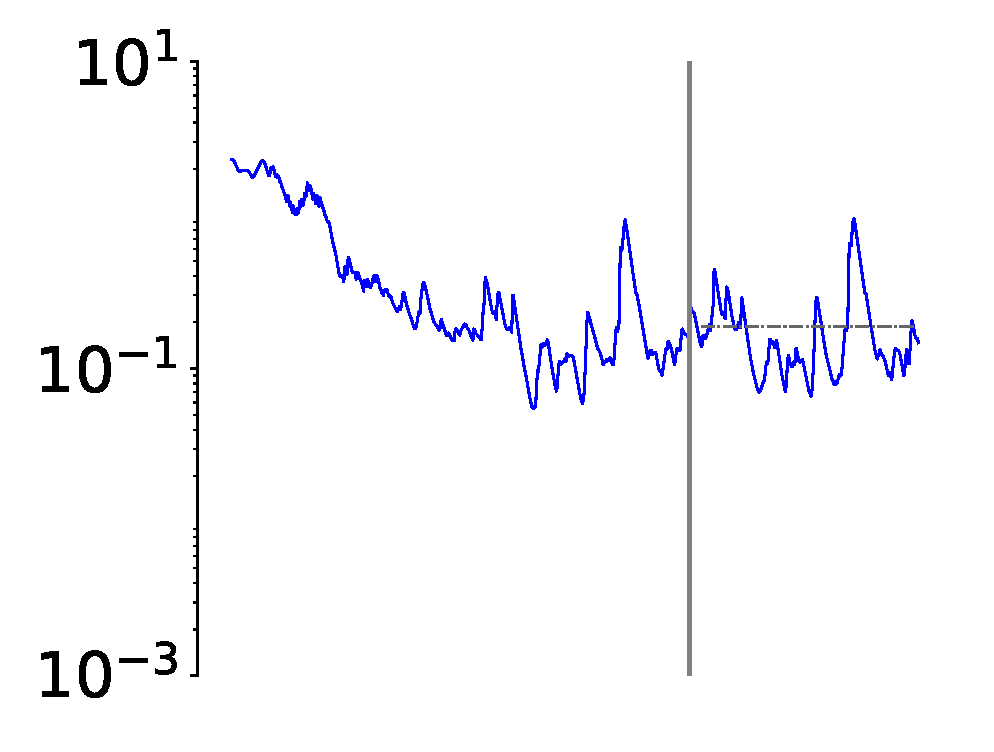
\includegraphics[height=0.15\linewidth,width=.45\linewidth]{Figures/Fig_T6/ImprovP/ST_T2_Seg9_Var_MSE.eps}
            \hspace{0em}
            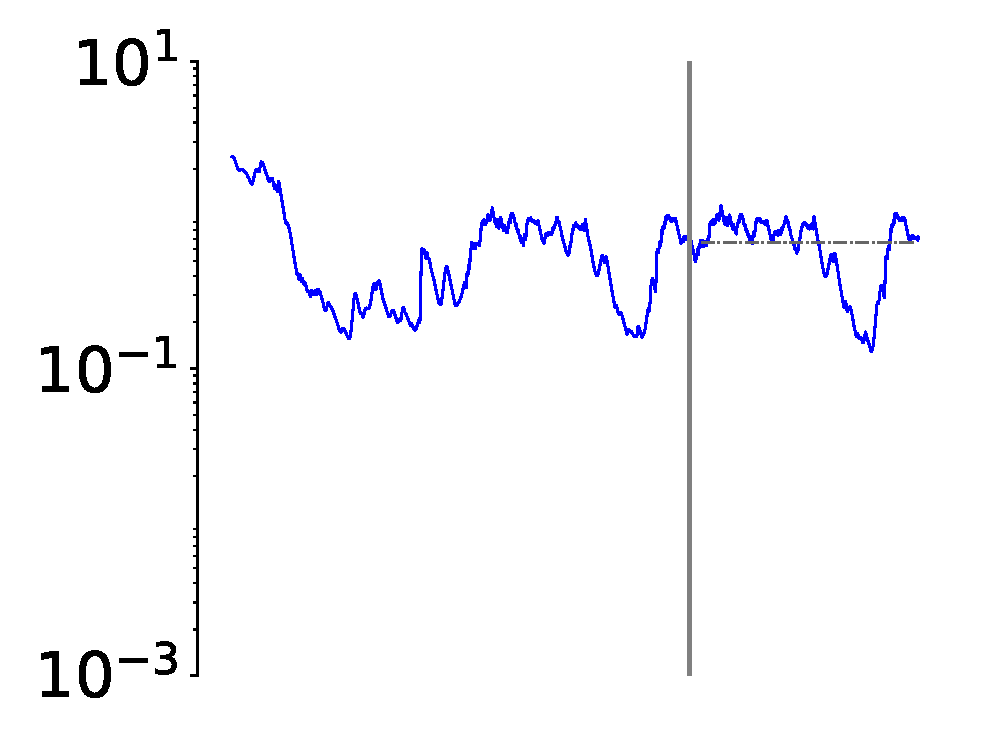
\includegraphics[height=0.15\linewidth,width=.45\linewidth]{Figures/Fig_T6/ImprovP/ST_T2_Seg10_Var_MSE.eps}
            
        \end{subfigure}
    \caption{Scalability of the performance of the modified Python re-implementation using the SUPERTREX algorithm on Task 2. The lengths of the arm segments are 1.8, 1.2 and 0.6 for the first three segments (akin to Task 3) and 0.1 for each additional segment. Here, the simulations for Task 2 with 5 to 50 segments are shown, all using the default seed 5489 for the random number generator. (Continued on next page.)}
    \label{Fig:Scalability_Task2}

\end{figure}
    
    
    
    
\begin{figure}
\ContinuedFloat
        \textbf{\rotatebox[origin=c]{90}{\hspace{-7.5em} MSE \hspace{2.5em} y(t) \hspace{1.5em} x(t)}}
        \begin{subfigure}{\textwidth}
            \centering
    
            \textbf{20 segments}\hspace{12em}\textbf{30 segments}
            
            
            
            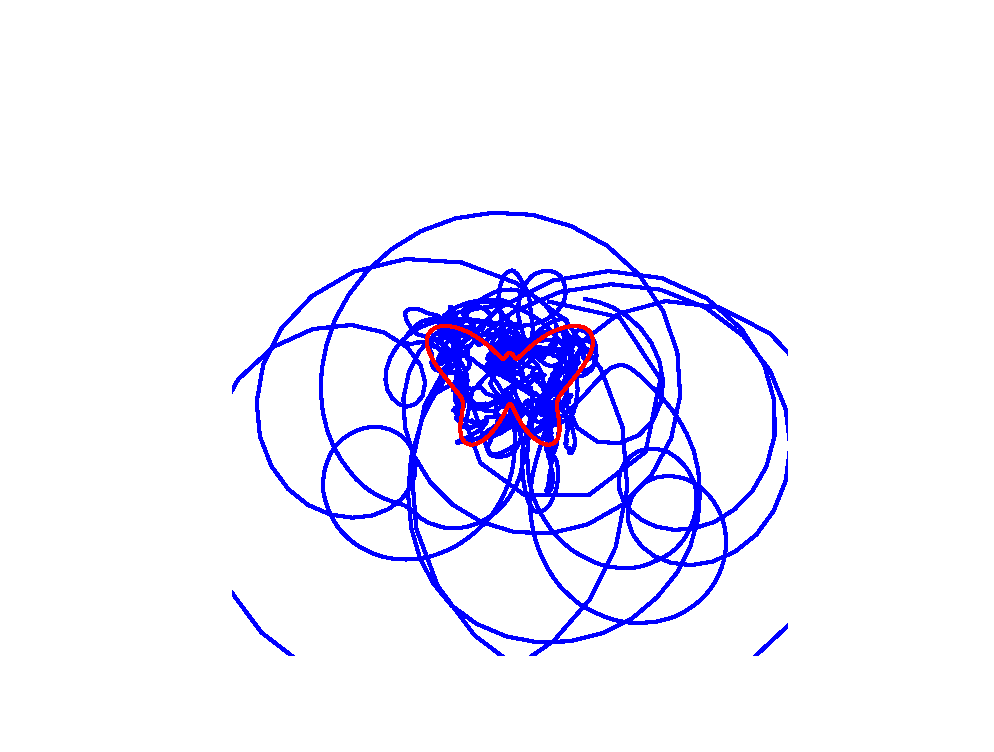
\includegraphics[trim=5cm 4cm 5cm 4cm, clip=true,height=0.15\linewidth]{Figures/Fig_T6/ImprovP/ST_T2_Seg20_Var_Trajectory.eps}
            \hspace{9em}
            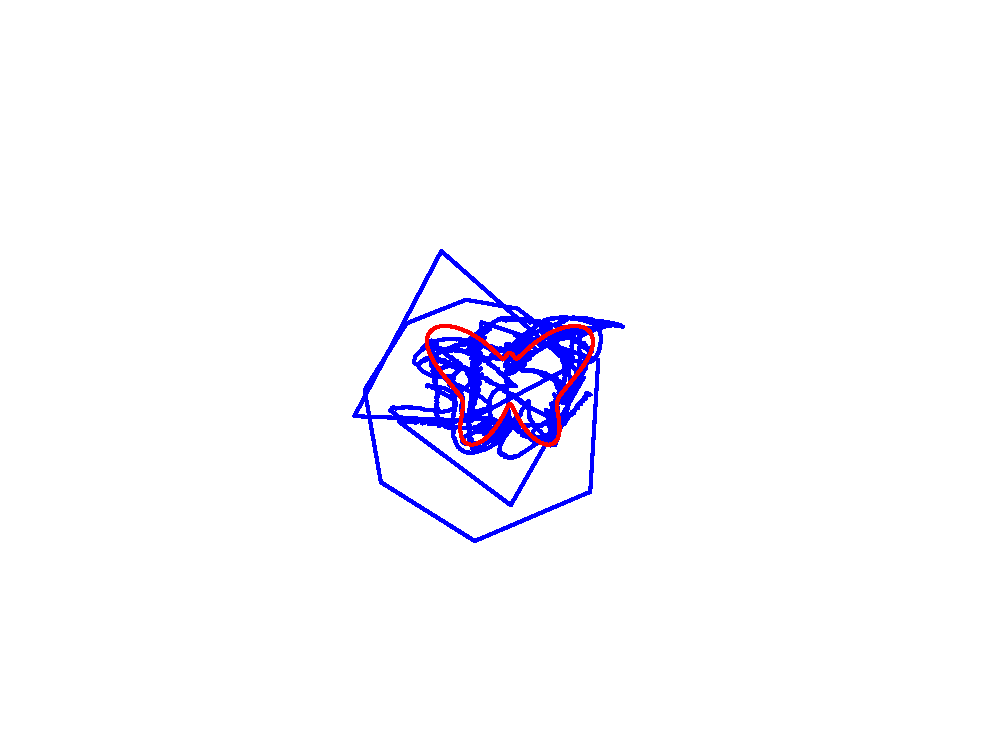
\includegraphics[trim=5cm 4cm 5cm 4cm, clip=true,height=0.15\linewidth]{Figures/Fig_T6/ImprovP/ST_T2_Seg30_Var_Trajectory.eps}
            %trim=1cm 0cm 0cm 0cm, clip=true,
            
            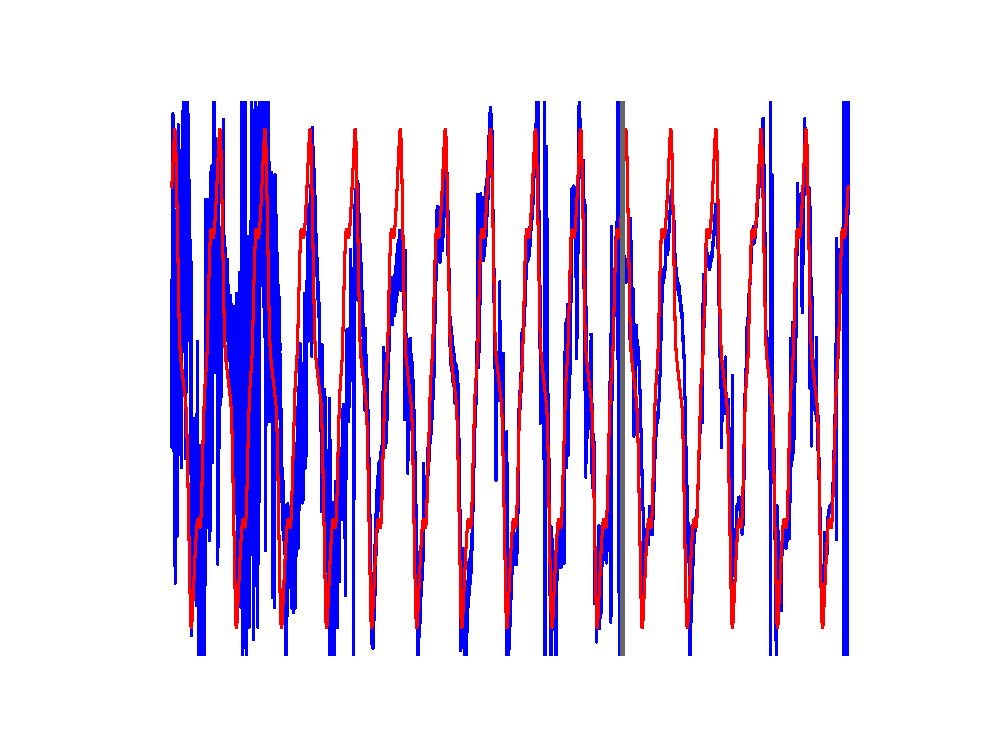
\includegraphics[trim=2cm 1cm 2cm 1cm, clip=true,height=0.1\linewidth,width=.45\linewidth]{Figures/Fig_T6/ImprovP/ST_T2_Seg20_Var_CoordinateX.eps} 
            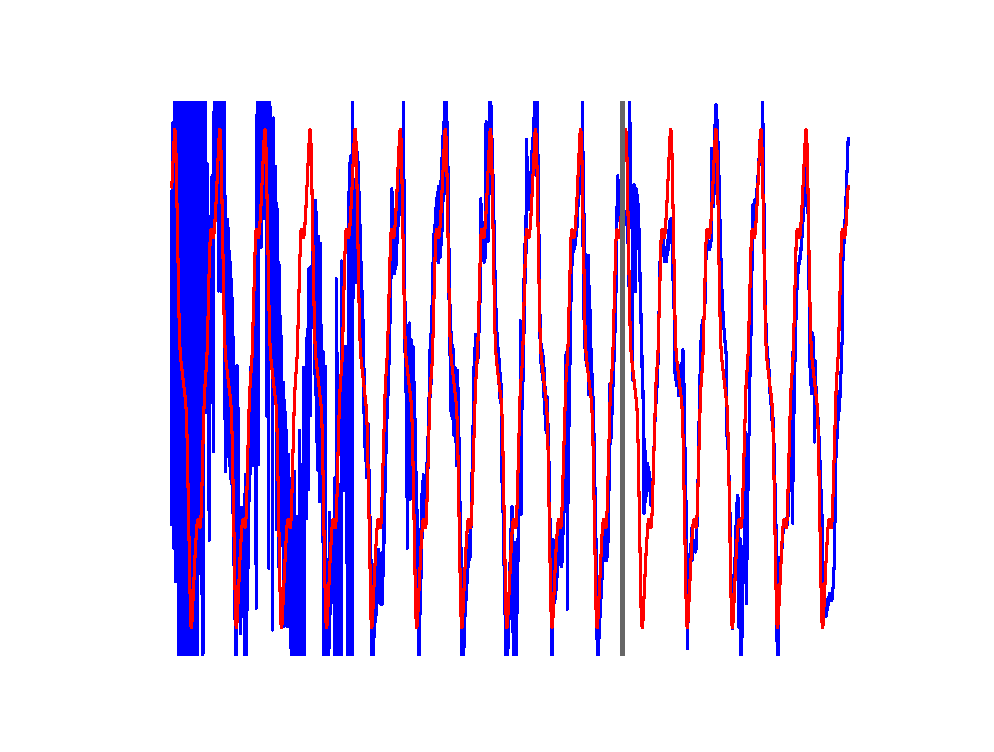
\includegraphics[trim=2cm 1cm 2cm 1cm, clip=true,height=0.1\linewidth,width=.45\linewidth]{Figures/Fig_T6/ImprovP/ST_T2_Seg30_Var_CoordinateX.eps}       

            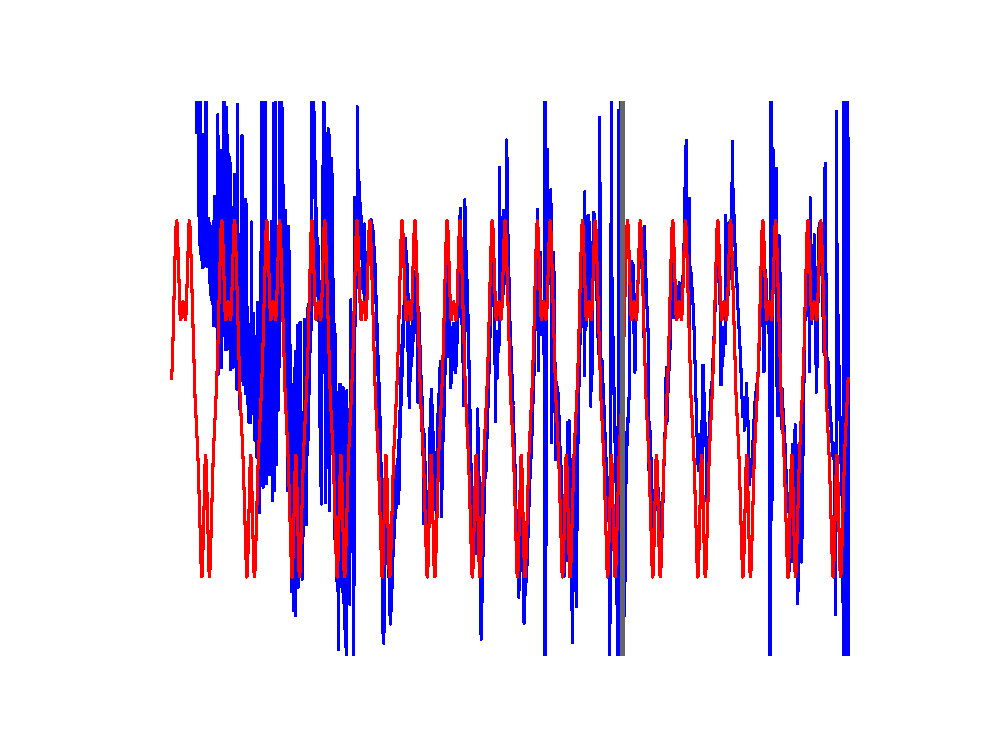
\includegraphics[trim=2cm 1cm 2cm 1cm, clip=true,height=0.1\linewidth,width=.45\linewidth]{Figures/Fig_T6/ImprovP/ST_T2_Seg20_Var_CoordinateY.eps}    
            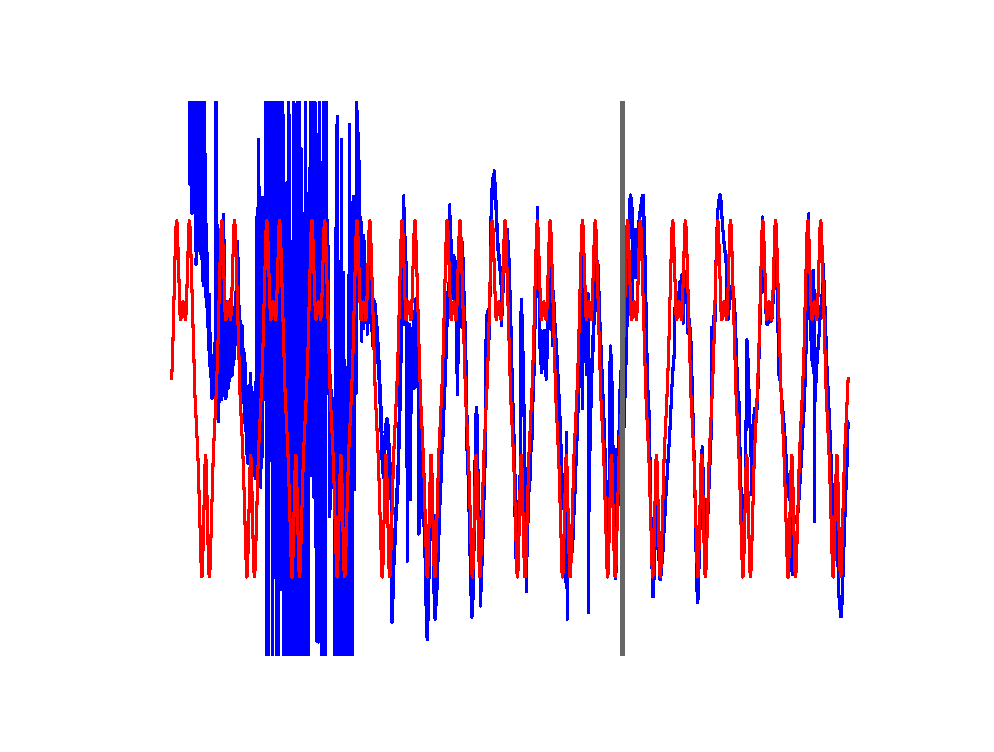
\includegraphics[trim=2cm 1cm 2cm 1cm, clip=true,height=0.1\linewidth,width=.45\linewidth]{Figures/Fig_T6/ImprovP/ST_T2_Seg30_Var_CoordinateY.eps} 

            \hspace{-1em}
            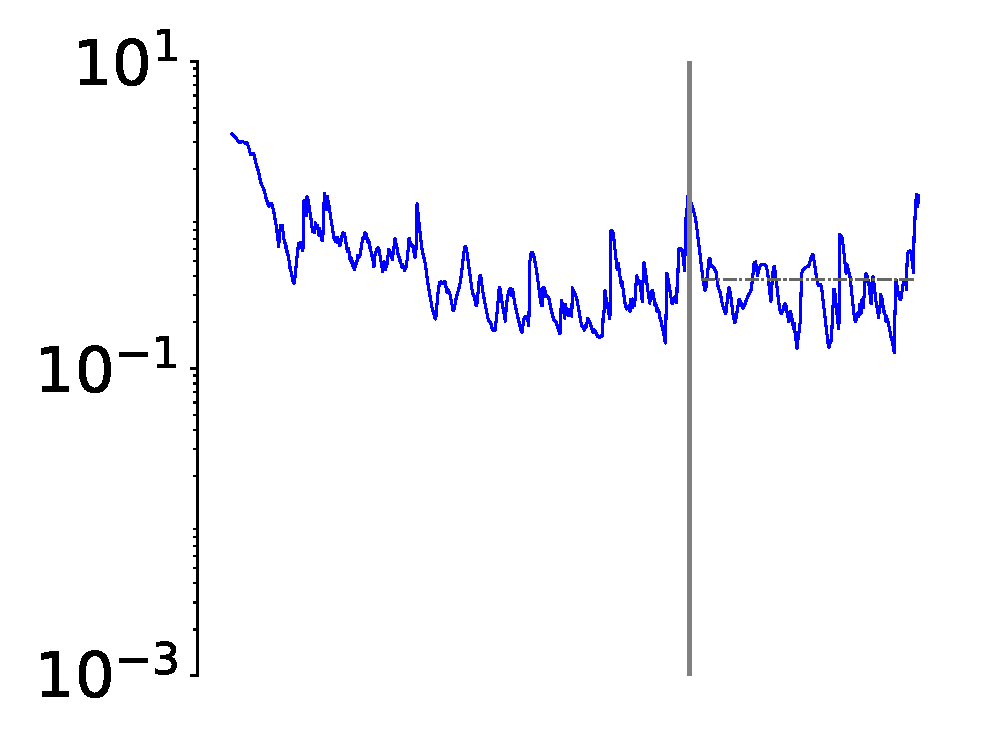
\includegraphics[height=0.15\linewidth,width=.45\linewidth]{Figures/Fig_T6/ImprovP/ST_T2_Seg20_Var_MSE.eps}
            \hspace{0em}
            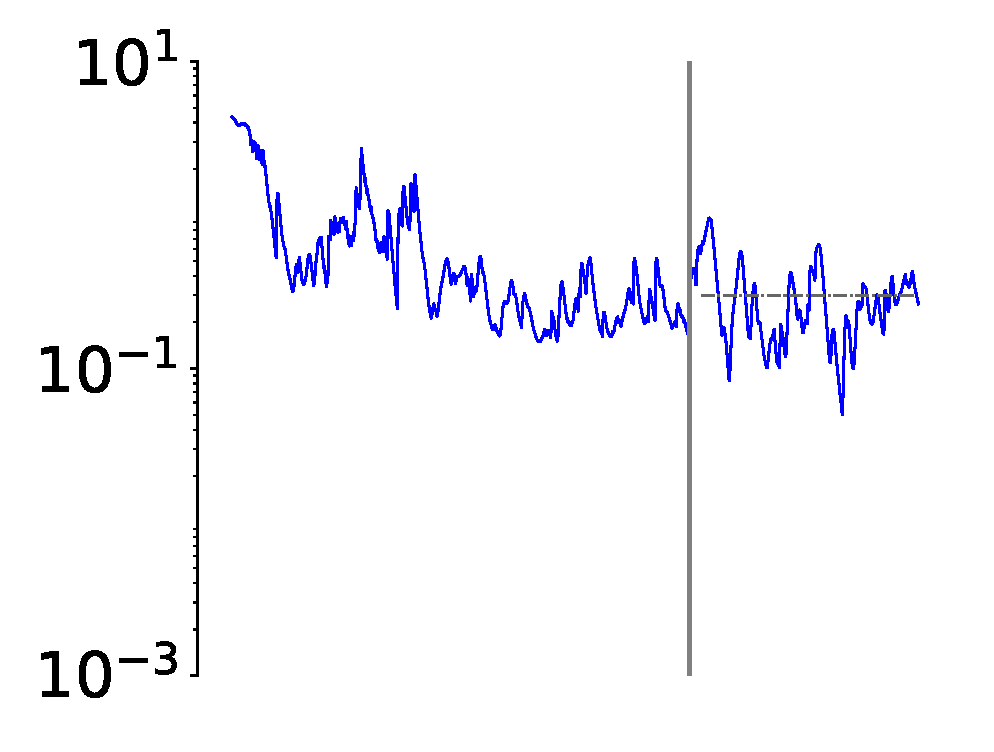
\includegraphics[height=0.15\linewidth,width=.45\linewidth]{Figures/Fig_T6/ImprovP/ST_T2_Seg30_Var_MSE.eps}
            
        \end{subfigure}
        
        \textbf{\rotatebox[origin=c]{90}{\hspace{-7.5em} MSE \hspace{2.5em} y(t) \hspace{1.5em} x(t)}}
        \begin{subfigure}{\textwidth}
            \centering
    
            \textbf{40 segments}\hspace{12em}\textbf{50 segments}
            
            
            
            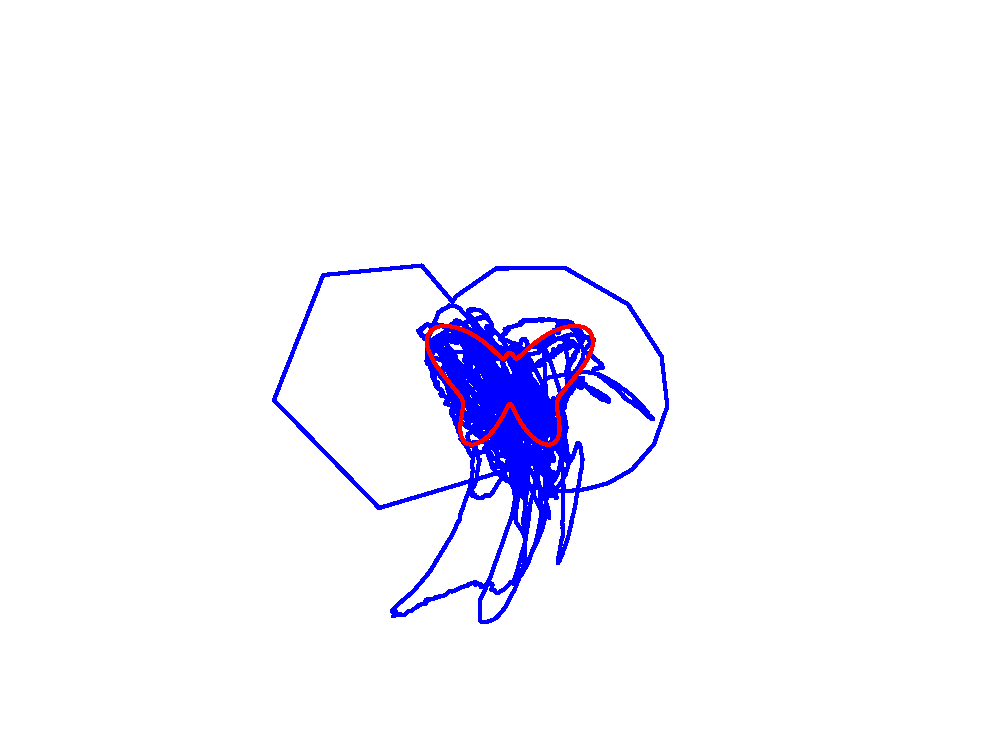
\includegraphics[trim=5cm 4cm 5cm 4cm, clip=true,height=0.15\linewidth]{Figures/Fig_T6/ImprovP/ST_T2_Seg40_Var_Trajectory.eps}
            \hspace{9em}
            \includegraphics[trim=5cm 4cm 5cm 4cm, clip=true,height=0.15\linewidth]{Figures/Fig_T6/ImprovP/ST_T2_Seg50_Var_Trajectory.eps}
            %trim=1cm 0cm 0cm 0cm, clip=true,
            
            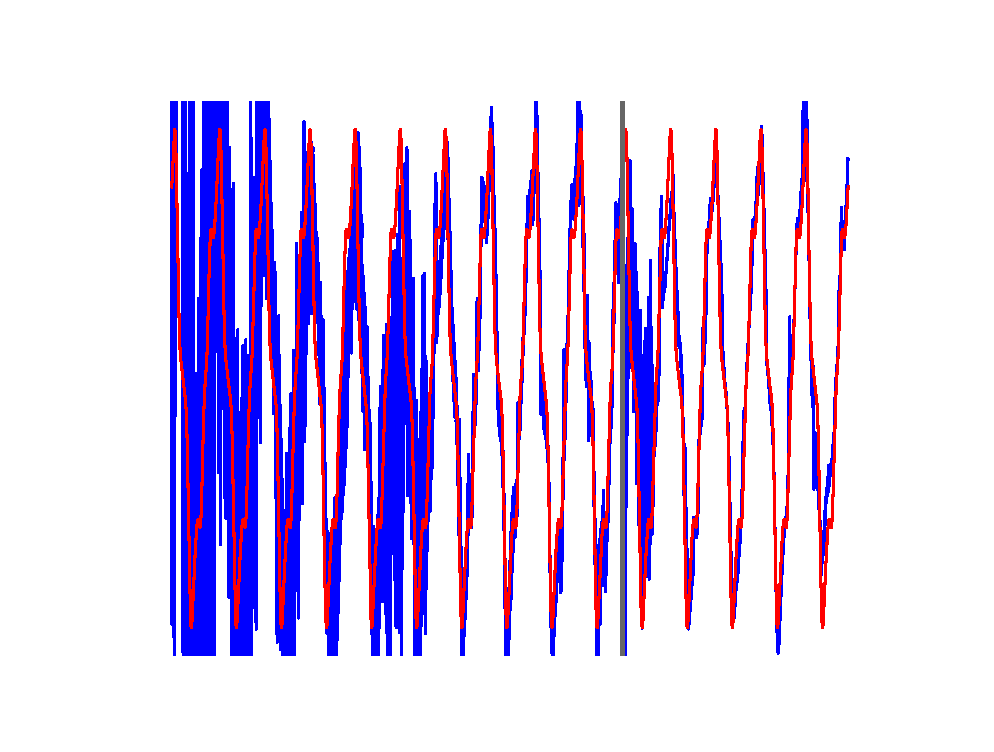
\includegraphics[trim=2cm 1cm 2cm 1cm, clip=true,height=0.1\linewidth,width=.45\linewidth]{Figures/Fig_T6/ImprovP/ST_T2_Seg40_Var_CoordinateX.eps} 
            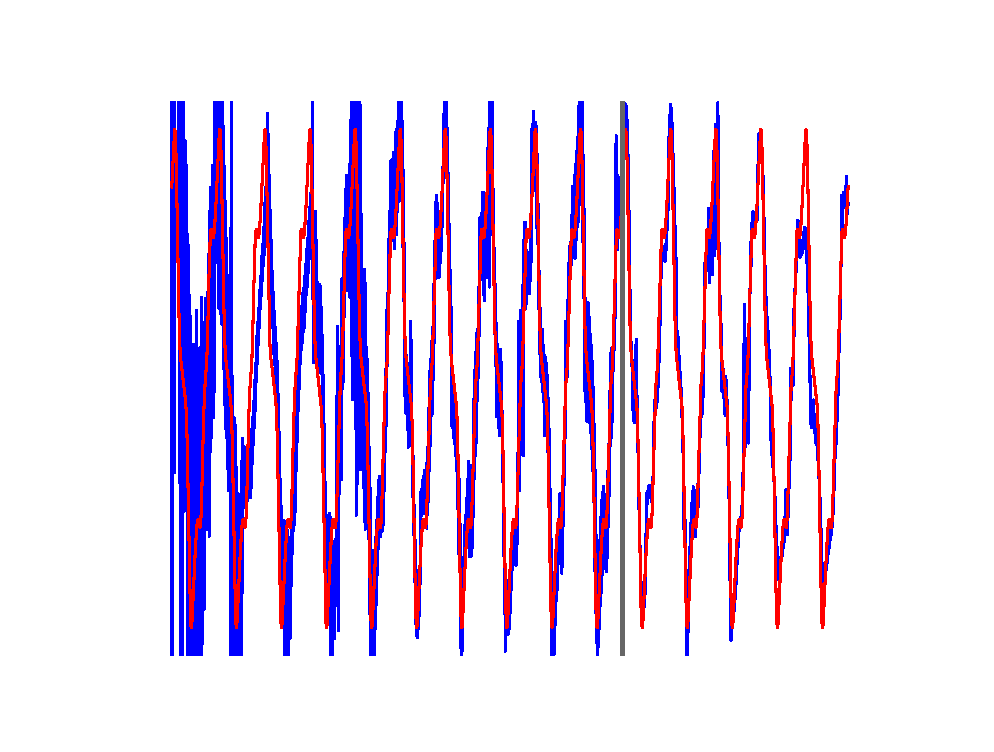
\includegraphics[trim=2cm 1cm 2cm 1cm, clip=true,height=0.1\linewidth,width=.45\linewidth]{Figures/Fig_T6/ImprovP/ST_T2_Seg50_Var_CoordinateX.eps}       

            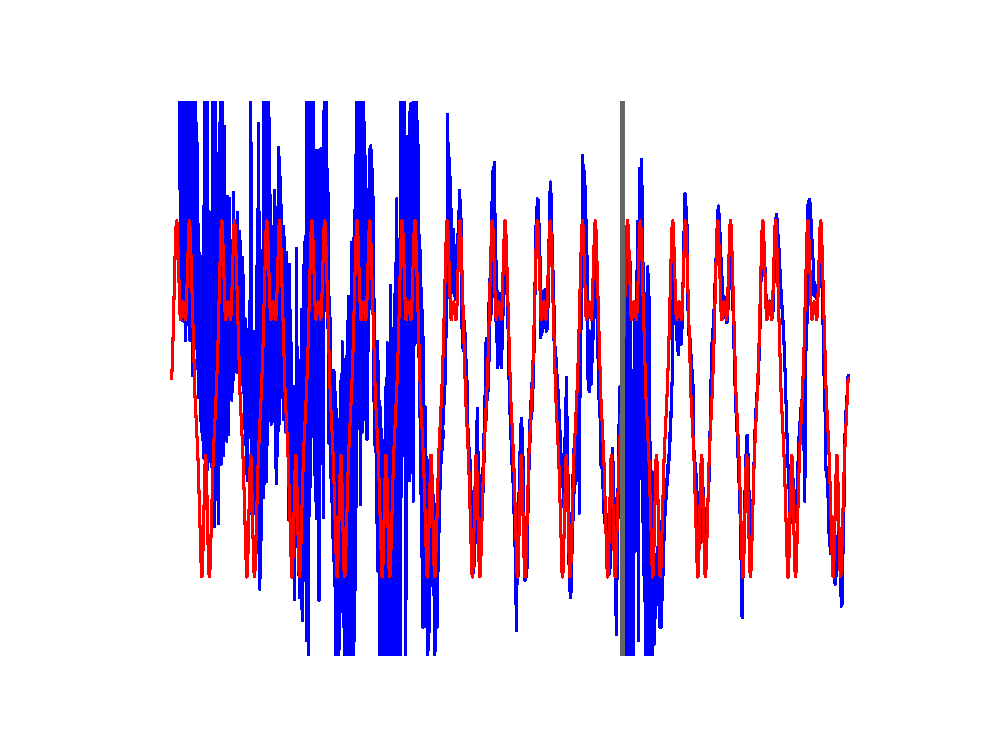
\includegraphics[trim=2cm 1cm 2cm 1cm, clip=true,height=0.1\linewidth,width=.45\linewidth]{Figures/Fig_T6/ImprovP/ST_T2_Seg40_Var_CoordinateY.eps}    
            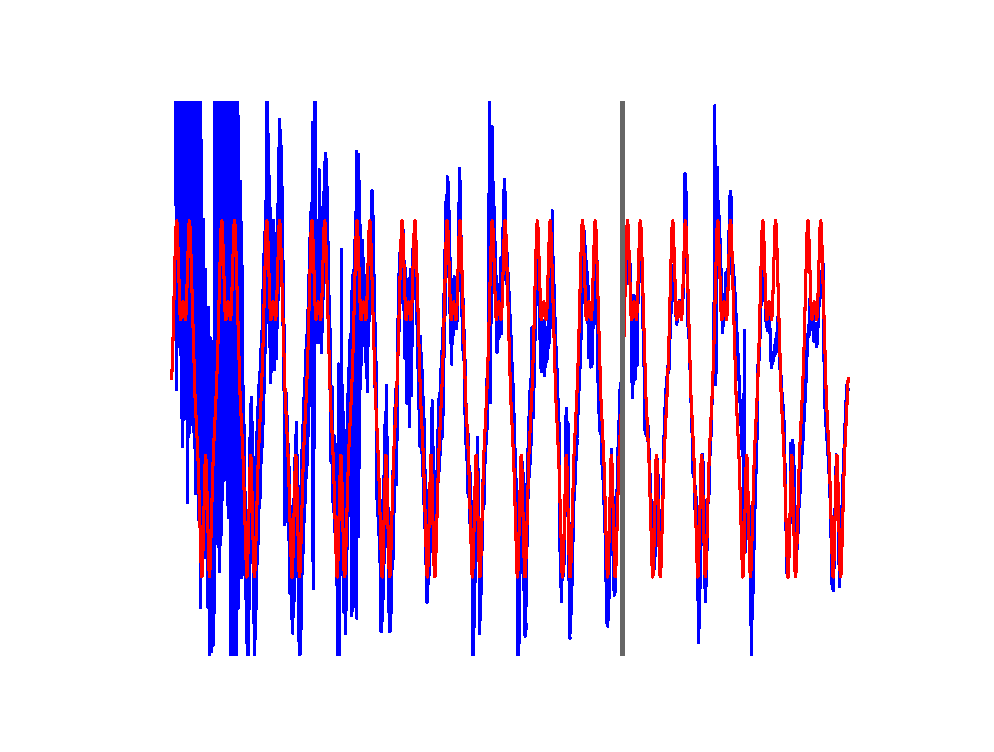
\includegraphics[trim=2cm 1cm 2cm 1cm, clip=true,height=0.1\linewidth,width=.45\linewidth]{Figures/Fig_T6/ImprovP/ST_T2_Seg50_Var_CoordinateY.eps} 

            \hspace{-1em}
            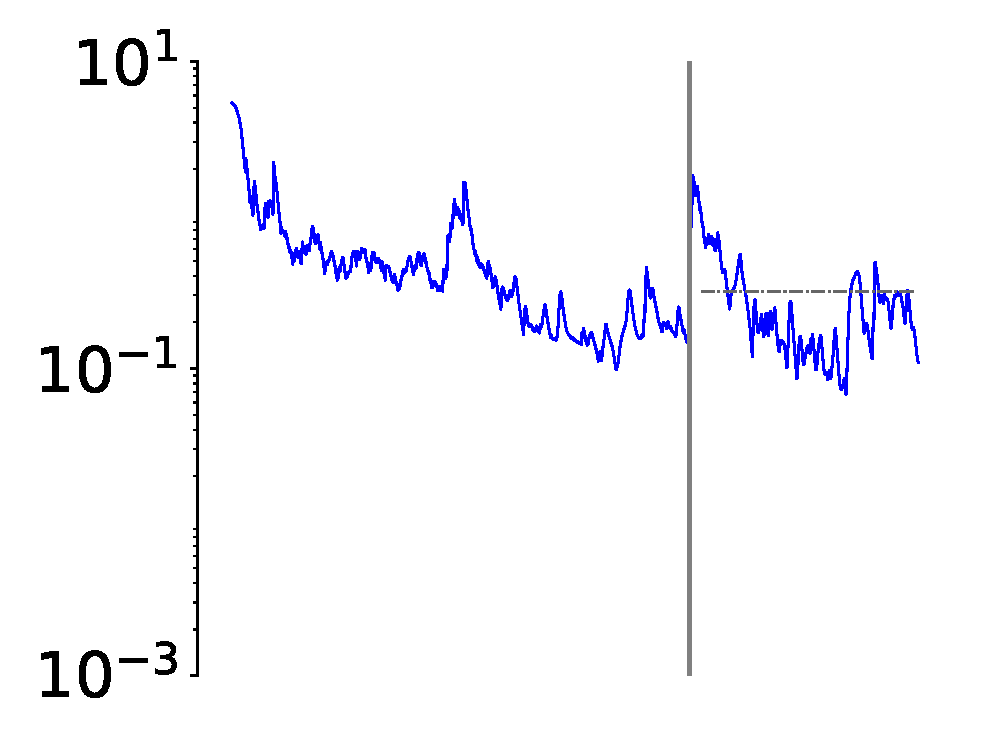
\includegraphics[height=0.15\linewidth,width=.45\linewidth]{Figures/Fig_T6/ImprovP/ST_T2_Seg40_Var_MSE.eps}
            \hspace{0em}
            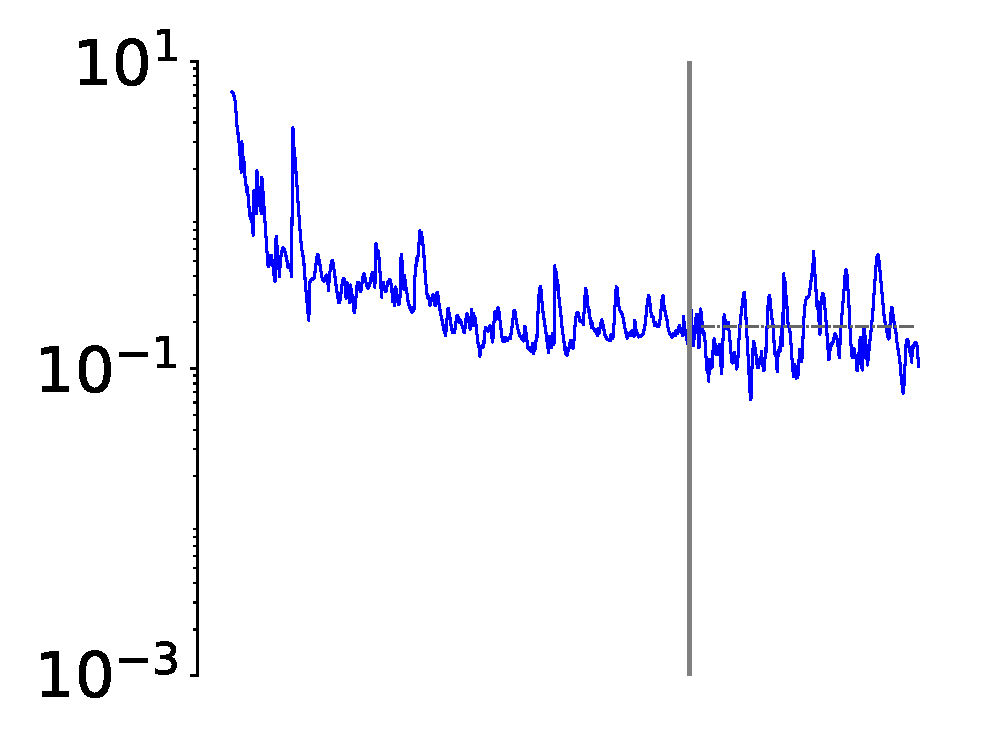
\includegraphics[height=0.15\linewidth,width=.45\linewidth]{Figures/Fig_T6/ImprovP/ST_T2_Seg50_Var_MSE.eps}
            
        \end{subfigure}
        
        
        
    
        
        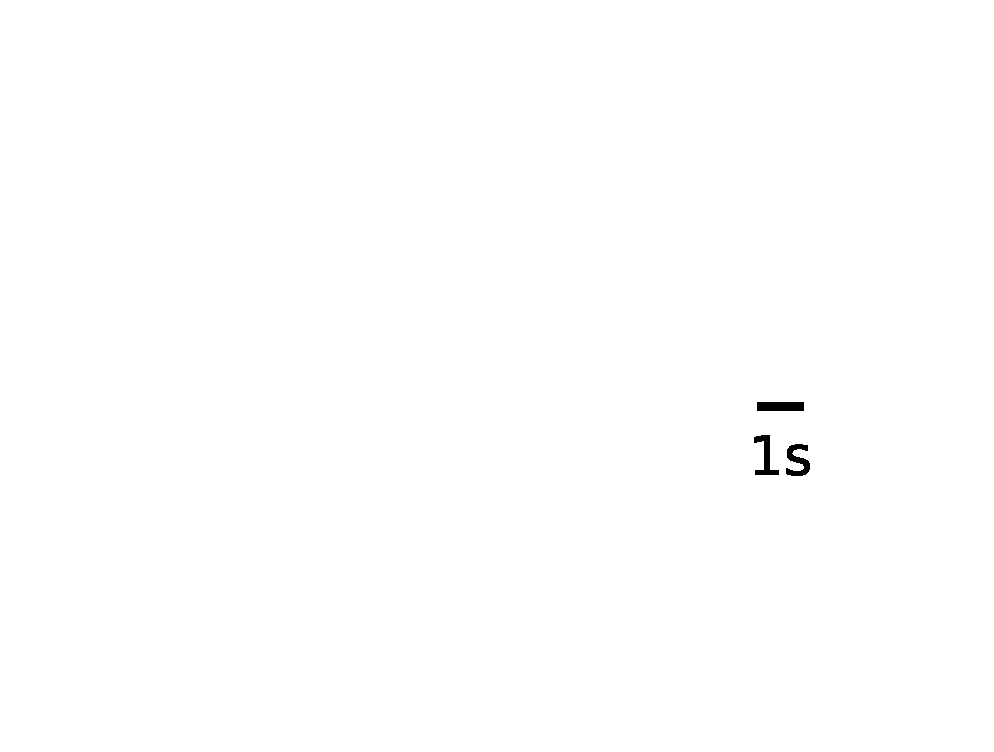
\includegraphics[trim=2cm 6cm 2cm 6cm, clip=true,height=0.05\linewidth,width=.4\linewidth]{Figures/Fig_T1/Python/ST_T1_Scale.eps}
        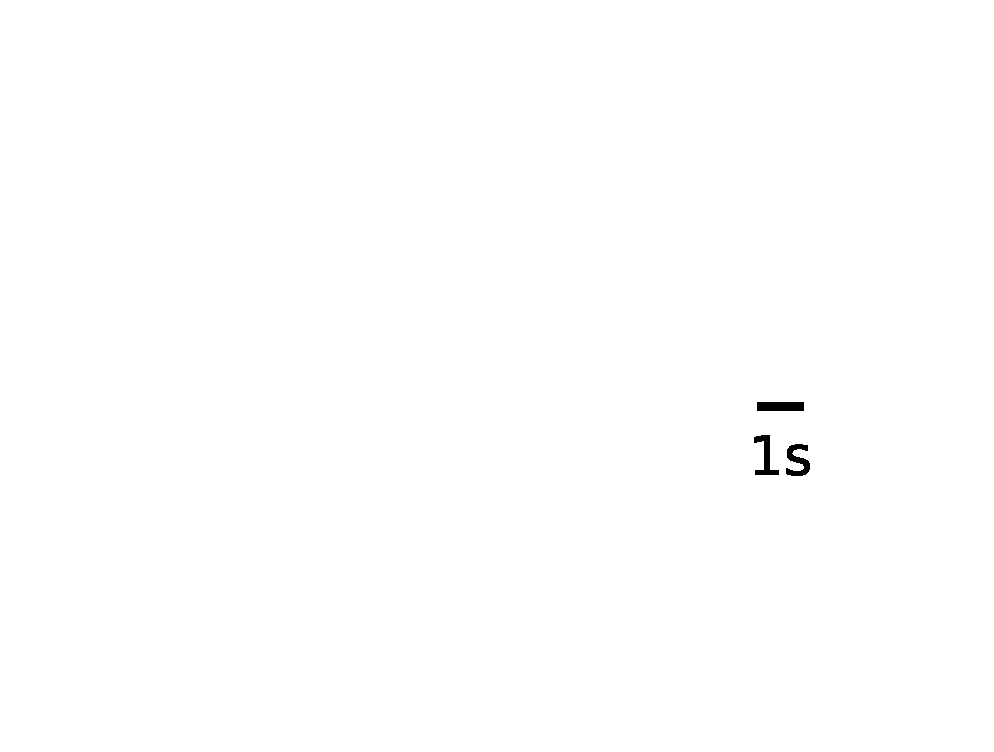
\includegraphics[trim=2cm 4cm 2cm 6cm, clip=true,height=0.05\linewidth,width=.45\linewidth]{Figures/Fig_T1/Python/ST_T1_Scale.eps}
    


    \caption{(Continued from previous page.) Scalability of the performance of the modified Python re-implementation using the SUPERTREX algorithm on Task 2. The lengths of the arm segments are 1.8, 1.2 and 0.6 for the first three segments (akin to Task 3) and 0.1 for each additional segment. Here, the simulations for Task 2 with 5 to 50 segments are shown, all using the default seed 5489 for the random number generator. In each subfigure, the top panel shows the produced trajectory, the middle panels show the evolution of the x and y coordinates of the end-effector of the arm (blue) throughout the training and test phase, along with the target coordinates (red). The grey vertical line marks the separation of the training and testing phase. The bottom panel shows the progression of the distance from target metric (blue) over the simulation, using the log scale for the y axis. The horizontal grey line, in the test phase, indicates the deviation metric.}
    \label{Fig:Scalability_Task2_cont}

\end{figure}
